\chapter{Requirement Analysis}
\label{chap:requirements}

\begin{chapterintro}
This chapter describes one of the most important stages in software development: the requirement analysis using different scenarios. For this, a detailed analysis of the possible use cases is made using the Unified Modeling Language (UML). This language allows us to specify, build and document a system using graphic language. 
\end{chapterintro}


\cleardoublepage

\section{Overview}
The result of this chapter will be a complete specification of the requirements, which will be matched by each module in the design stage. This helps us also to focus on key aspects and take apart other less important functionalities that could be implemented in future works.

%As commented before, our project aims to develop a personal assistance system that integrates the advantages of agent systems, information retrieval and Natural Language Processing. Our personal assistant should have the capability to solve user's questions using all of these features.

\section{Use cases}

These sections identify the use cases of the system. This helps us to obtain a complete specification of the uses of the system, and therefore define the complete list of requisites to match.  First, we will present a list of the actors in the system and a UML diagram representing all the actors participating in the different use cases. This representation allows, apart from specifying the actors that interact in the system, the relationships between them.

These use cases will be described the next sections, including each one a table with their complete specification. Using these tables, we will be able to define the requirements to be established.


\subsection{Actors dictionary}

\noindent The list of primary and secondary actors is presented in table \ref{tab:actores}. These actors participate in the different use cases, which are presented later.\\



\begin{table}[!htpb]
\centering
\begin{tabular}{|c|c|x{6cm}|}
\noalign{\hrule height 2pt}
\textbf{Actor identifier} & \textbf{Role} & \textbf{Description}\tn
\hline
ACT-1 & Gamer & End user that play the game using the physical instruments and the application\tn
\hline
ACT-2 & Instrument recognition algorithm & Algorithm that detects what physical figure has been placed on the application recognition zones\tn
\hline
ACT-3 & Client & Company that have outsourced the game development\tn
\hline
ACT-4 & Flurry & Tecnhology that manage application metrics and errors\tn
\noalign{\hrule height 2pt}
\end{tabular}
\caption{Actors list}
\label{tab:actores}
\end{table}


\clearpage


\FloatBarrier


\subsection{Game modes use case}
\label{subsec:gamemodes}
This use case package collects the game play modes and their functionalities, as shown in \ref{fig:pack-uc1}.

The use cases presented in this section are as shown in the Figure \ref{fig:pack-uc1}:
\begin{itemize}
\item \textit{play instrument} detailed in sub-section \ref{subsec:playinstrument}.
\item \textit{conducte orchestra} detailed in sub-section \ref{subsec:conducteorchestra}.
\item \textit{discover instrument}  detailed in sub-section \ref{subsec:discoverinstrument}.
\item \textit{watch demo}  detailed in sub-section \ref{subsec:watchdemo}.
\item \textit{select melody}  detailed in sub-section \ref{subsec:selectmelody}.
\item \textit{select instrument}  detailed in sub-section \ref{subsec:selectinstrument}.
\end{itemize}


\begin{figure}[h]
\centering
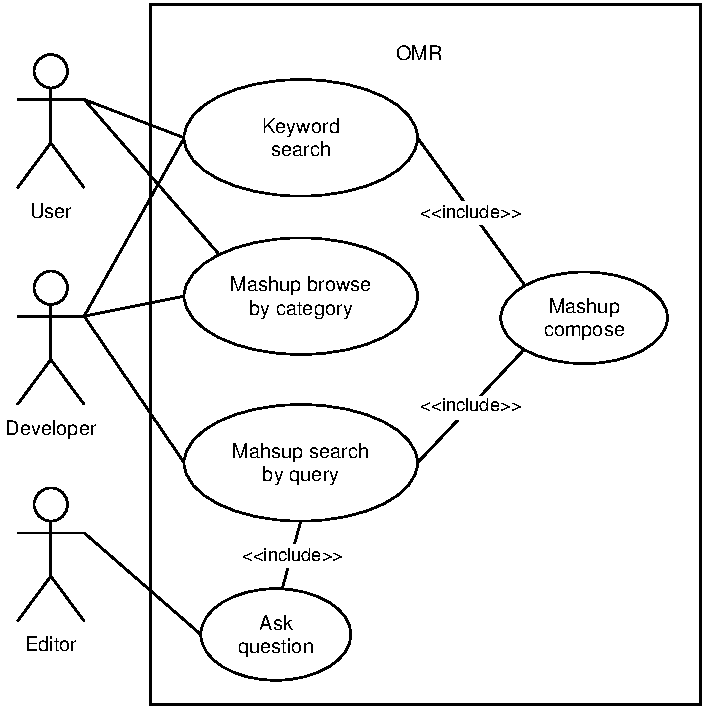
\includegraphics[width=400pt]{graphics/uc1.pdf}
\caption{Game modes use case}
\label{fig:pack-uc1}
\end{figure}

\newpage
\subsubsection{Play instrument}
\label{subsec:playinstrument}

\begin{table}[!htpb]
\centering
\begin{tabular}{|c|x{1cm}x{5cm}x{5cm}|}
\noalign{\hrule height 2pt}
\textbf{Use Case Name} & \multicolumn{3}{c|}{play instrument}\\
\hline
\textbf{Use Case ID} & \multicolumn{3}{x{11cm}|}{UC1.1}\\
\hline
\textbf{Primary Actor} & \multicolumn{3}{c|}{Gamer}\\
\hline
\textbf{Pre-Condition} & \multicolumn{3}{x{11cm}|}{The application is showing the home screen and the gamer has the instruments physical miniatures}\\
\hline
\textbf{Post-Condition} & \multicolumn{3}{x{11cm}|}{Optionally, the gamer can watch a demo, change the instrument or change the melody}\\
\hline
\textbf{Flow of Events} & \multicolumn{1}{c|}{} & \multicolumn{1}{x{5cm}|}{Actor Input} & \multicolumn{1}{x{5cm}|}{System Response}\\
\hline

\textbf{} & \multicolumn{1}{x{0.5cm}|}{1} & \multicolumn{1}{x{5cm}|}{The gamer put an instrument miniature on home screen. The instrument is placed in the detection zone circle that represents the play instrument game mode} & \multicolumn{1}{x{5cm}|}{The application load the play instrument mode game with the instrument that have been placed on the screen and the default melody. }\\
\hline

\end{tabular}
\end{table}

\FloatBarrier

\newpage
\subsubsection{Conducte orchestra}
\label{subsec:conducteorchestra}


\begin{table}[!htpb]
\centering
\begin{tabular}{|c|x{1cm}x{5cm}x{5cm}|}
\noalign{\hrule height 2pt}
\textbf{Use Case Name} & \multicolumn{3}{c|}{conducte orchestra}\\
\hline
\textbf{Use Case ID} & \multicolumn{3}{x{11cm}|}{UC1.2}\\
\hline
\textbf{Primary Actor} & \multicolumn{3}{c|}{Gamer}\\
\hline
\textbf{Pre-Condition} & \multicolumn{3}{x{11cm}|}{The application is showing the home screen and the gamer has the instruments physical miniatures}\\
\hline
\textbf{Post-Condition} & \multicolumn{3}{x{11cm}|}{Optionally, the gamer can play, stop or change the melody, enable or disable an instrument and change the instrument family}\\
\hline
\textbf{Flow of Events} & \multicolumn{1}{c|}{} & \multicolumn{1}{x{5cm}|}{Actor Input} & \multicolumn{1}{x{5cm}|}{System Response}\\
\hline

\textbf{} & \multicolumn{1}{x{0.5cm}|}{1} & 
\multicolumn{1}{x{5cm}|}{The gamer put an instrument miniature on home screen. The instrument is placed in the detection zone circle that represents the conduct orchestra game mode} & 
\multicolumn{1}{x{5cm}|}{The application load the conduct orchestra game mode with all instruments enabled, the family instrument selector of the family instrument that have been placed on the screen enabled, and the default melody.}\\
\hline

\end{tabular}
\end{table}
\FloatBarrier

\newpage
\subsubsection{Discover instrument}
\label{subsec:discoverinstrument}

\FloatBarrier

\begin{table}[!htpb]
\centering
\begin{tabular}{|c|x{1cm}x{5cm}x{5cm}|}
\noalign{\hrule height 2pt}
\textbf{Use Case Name} & \multicolumn{3}{c|}{discover instrument}\\
\hline
\textbf{Use Case ID} & \multicolumn{3}{x{11cm}|}{UC1.3}\\
\hline
\textbf{Primary Actor} & \multicolumn{3}{c|}{Gamer}\\
\hline
\textbf{Pre-Condition} & \multicolumn{3}{x{11cm}|}{The application is showing the home screen and the gamer has the instruments physical miniatures}\\
\hline
\textbf{Post-Condition} & \multicolumn{3}{x{11cm}|}{Optionally, the gamer can play the an instrument sound and change the instrument family}\\
\hline
\textbf{Flow of Events} & \multicolumn{1}{c|}{} & \multicolumn{1}{x{5cm}|}{Actor Input} & \multicolumn{1}{x{5cm}|}{System Response}\\
\hline

\textbf{} & \multicolumn{1}{x{0.5cm}|}{1} & 
\multicolumn{1}{x{5cm}|}{The gamer put an instrument miniature on home screen. The instrument is placed in the detection zone circle that represents the discover instrument game mode} & 
\multicolumn{1}{x{5cm}|}{The application load the discover instrument game mode with the instruments of the family instrument that have been placed on the screen. The game mode shows instrument information and sounds}\\
\hline

\end{tabular}
\end{table}

\FloatBarrier

\newpage
\subsubsection{Watch demo}
\label{subsec:watchdemo}


\begin{table}[!htpb]
\centering
\begin{tabular}{|c|x{1cm}x{5cm}x{5cm}|}
\noalign{\hrule height 2pt}
\textbf{Use Case Name} & \multicolumn{3}{c|}{watch demo}\\
\hline
\textbf{Use Case ID} & \multicolumn{3}{x{11cm}|}{UC1.4}\\
\hline
\textbf{Primary Actor} & \multicolumn{3}{c|}{Gamer}\\
\hline
\textbf{Pre-Condition} & \multicolumn{3}{x{11cm}|}{Play instrument game mode has been selected}\\
\hline
\textbf{Post-Condition} & \multicolumn{3}{x{11cm}|}{-}\\
\hline
\textbf{Flow of Events} & \multicolumn{1}{c|}{} & \multicolumn{1}{x{5cm}|}{Actor Input} & \multicolumn{1}{x{5cm}|}{System Response}\\
\hline

\textbf{} & \multicolumn{1}{x{0.5cm}|}{1} & 
\multicolumn{1}{x{5cm}|}{The gamer touch Demo button with a selected melody and instrument} & 
\multicolumn{1}{x{5cm}|}{The melody in played with the instrument selected and musical notes are highlated}\\
\hline


\end{tabular}
\end{table}
\FloatBarrier

\newpage
\subsubsection{Select melody}
\label{subsec:selectmelody}

\begin{table}[!htpb]
\centering
\begin{tabular}{|c|x{1cm}x{5cm}x{5cm}|}
\noalign{\hrule height 2pt}
\textbf{Use Case Name} & \multicolumn{3}{c|}{select melody}\\
\hline
\textbf{Use Case ID} & \multicolumn{3}{x{11cm}|}{UC1.5}\\
\hline
\textbf{Primary Actor} & \multicolumn{3}{c|}{Gamer}\\
\hline
\textbf{Pre-Condition} & \multicolumn{3}{x{11cm}|}{Play instrument game mode or conduct orchestra have been selected}\\
\hline
\textbf{Post-Condition} & \multicolumn{3}{x{11cm}|}{-}\\
\hline
\textbf{Flow of Events} & \multicolumn{1}{c|}{} & \multicolumn{1}{x{5cm}|}{Actor Input} & \multicolumn{1}{x{5cm}|}{System Response}\\
\hline

\textbf{} & \multicolumn{1}{x{0.5cm}|}{1} & 
\multicolumn{1}{x{5cm}|}{The gamer touch Melodies button} & 
\multicolumn{1}{x{5cm}|}{A list of the melodies are shown}\\
\hline

\textbf{} & \multicolumn{1}{x{0.5cm}|}{2} & 
\multicolumn{1}{x{5cm}|}{The gamer chose one of the avaiable melodies} & 
\multicolumn{1}{x{5cm}|}{Selected melody is loaded into game mode}\\
\hline

\end{tabular}
\end{table}
\FloatBarrier

\newpage
\subsubsection{Select instrument}
\label{subsec:selectinstrument}

\begin{table}[!htpb]
\centering
\begin{tabular}{|c|x{1cm}x{5cm}x{5cm}|}
\noalign{\hrule height 2pt}
\textbf{Use Case Name} & \multicolumn{3}{c|}{select instrument}\\
\hline
\textbf{Use Case ID} & \multicolumn{3}{x{11cm}|}{UC1.6}\\
\hline
\textbf{Primary Actor} & \multicolumn{3}{c|}{Gamer}\\
\hline
\textbf{Secondary Actor} & \multicolumn{3}{c|}{Instrument recognition algorithm}\\
\hline
\textbf{Pre-Condition} & \multicolumn{3}{x{11cm}|}{Any game mode is selected and the gamer has the instruments physical miniatures}\\
\hline
\textbf{Post-Condition} & \multicolumn{3}{x{11cm}|}{O-}\\
\hline
\textbf{Flow of Events} & \multicolumn{1}{c|}{} & \multicolumn{1}{x{5cm}|}{Actor Input} & \multicolumn{1}{x{5cm}|}{System Response}\\
\hline

\textbf{} & \multicolumn{1}{x{0.5cm}|}{1} & 
\multicolumn{1}{x{5cm}|}{The Gamer place the instrument in the circle recognition zone} & 
\multicolumn{1}{x{5cm}|}{The Instrument recognition algorithm process the instrument pad touches and determine which instrument have been placed}\\
\hline

\textbf{} & \multicolumn{1}{x{0.5cm}|}{2} & 
\multicolumn{1}{x{5cm}|}{The Instrument recognition algorithm detect a different instrument} & 
\multicolumn{1}{x{5cm}|}{Selected instrument is loaded into game mode}\\
\hline

\end{tabular}
\end{table}
\FloatBarrier

\newpage
\subsection{Game managment use case}
This use case package collects the main managment use cases of the game, as shown in \ref{fig:pack-uc2}

\begin{itemize}
\item \textit{metrics managment} detailed in subsection \ref{subsec:metricsmanagment}
\item \textit{errors managment} detailed in subsection \ref{subsec:errorsmanagment}
\end{itemize}

\begin{figure}[h]
\centering
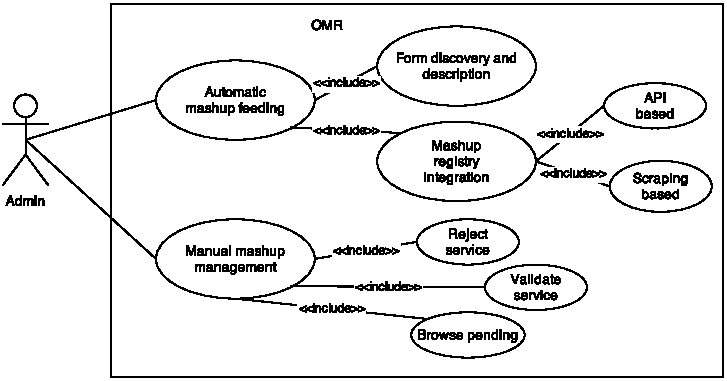
\includegraphics[width=400pt]{graphics/uc2.pdf}
\caption{Game managment use case}
\label{fig:pack-uc2}
\end{figure}

\FloatBarrier

\newpage
\subsubsection{Metrics managment}
\label{subsec:metricsmanagment}

\begin{table}[!htpb]
\centering
\begin{tabular}{|c|x{1cm}x{5cm}x{5cm}|}
\noalign{\hrule height 2pt}
\textbf{Use Case Name} & \multicolumn{3}{c|}{Metrics managment}\\
\hline
\textbf{Use Case ID} & \multicolumn{3}{x{11cm}|}{UC2.1}\\
\hline
\textbf{Primary Actor} & \multicolumn{3}{c|}{Client}\\
\hline
\textbf{Secondary Actor} & \multicolumn{3}{c|}{Flurry}\\
\hline
\textbf{Pre-Condition} & \multicolumn{3}{x{11cm}|}{Flurry client account has been created. Application is running}\\
\hline
\textbf{Post-Condition} & \multicolumn{3}{x{11cm}|}{Metrics are added to Flurry servers}\\
\hline
\textbf{Flow of Events} & \multicolumn{1}{c|}{} & \multicolumn{1}{x{5cm}|}{Actor Input} & \multicolumn{1}{x{5cm}|}{System Response}\\
\hline

\textbf{} & \multicolumn{1}{x{0.5cm}|}{1} & 
\multicolumn{1}{x{5cm}|}{The client access to their Flurry acount} & 
\multicolumn{1}{x{5cm}|}{Flurry shows all metrics included with their SDK in the application}\\
\hline

\end{tabular}
\end{table}
\FloatBarrier

\newpage
\subsubsection{Errors managment}
\label{subsec:errorsmanagment}

\begin{table}[!htpb]
\centering
\begin{tabular}{|c|x{1cm}x{5cm}x{5cm}|}
\noalign{\hrule height 2pt}
\textbf{Use Case Name} & \multicolumn{3}{c|}{Metrics managment}\\
\hline
\textbf{Use Case ID} & \multicolumn{3}{x{11cm}|}{UC2.2}\\
\hline
\textbf{Primary Actor} & \multicolumn{3}{c|}{Client/Developer}\\
\hline
\textbf{Secondary Actor} & \multicolumn{3}{c|}{Flurry}\\
\hline
\textbf{Pre-Condition} & \multicolumn{3}{x{11cm}|}{Flurry client and developer accounts has been created. Application is running and an error has been thrown}\\
\hline
\textbf{Post-Condition} & \multicolumn{3}{x{11cm}|}{Errors are sent to Flurry servers}\\
\hline
\textbf{Flow of Events} & \multicolumn{1}{c|}{} & \multicolumn{1}{x{5cm}|}{Actor Input} & \multicolumn{1}{x{5cm}|}{System Response}\\
\hline

\textbf{} & \multicolumn{1}{x{0.5cm}|}{1} & 
\multicolumn{1}{x{5cm}|}{The client and the developers access to their Flurry acount} & 
\multicolumn{1}{x{5cm}|}{Flurry shows all errors included with their SDK in the application}\\
\hline

\end{tabular}
\end{table}
\FloatBarrier

\subsection{Conclusions}

With the use cases described we have introduced the basic functionalities that have been implemented in this project. They help us to understand the different actors that can interact. They can serve as a base for further development and different use cases that can come to mind.